\documentclass{ctexart}
% \usepackage[UTF-8]{ctex}
\usepackage{amsmath}
\usepackage{booktabs}
\usepackage{multirow}
\usepackage{tabularx}
\usepackage{tabularx,booktabs,multirow,longtable}

\usepackage{booktabs,multirow,longtable}

\usepackage{listings}
\usepackage{listings}
\usepackage{color}

%导言区插入下面三行
\usepackage{graphicx} %插入图片的宏包
\usepackage{float} %设置图片浮动位置的宏包
\usepackage{subfigure} %插入多图时用子图显示的宏包


\definecolor{dkgreen}{rgb}{0,0.6,0}
\definecolor{gray}{rgb}{0.5,0.5,0.5}
\definecolor{mauve}{rgb}{0.58,0,0.82}

\lstset{frame=tb,
  language=Python,
  aboveskip=3mm,
  belowskip=3mm,
  showstringspaces=false,
  columns=flexible,
  basicstyle={\small\ttfamily},
  numbers=left,
  numberstyle=\tiny\color{gray},
  keywordstyle=\color{blue},
  commentstyle=\color{dkgreen},
  stringstyle=\color{mauve},
  breaklines=true,
  breakatwhitespace=true,
  tabsize=3
}


\title{作业2:数值求解泊松方程}
\author{谢文进}
\date{\today}
\begin{document}
\maketitle
\section{数值求解泊松方程}
\subsection{理论推导}
现求解二维泊松方程:
\begin{equation}%要调用宏包amsmath
    \begin{cases}
        \frac{\partial^2 u}{\partial x^2} + \frac{\partial^2 u}{\partial y^2} = f(x,y), \quad (x, y)\in \Omega\\
        u = u_0 \quad \text{on} \ \partial \Omega
    \end{cases}	
\end{equation}
其中区域$\Omega$为矩形区域,即$\Omega=\{(x,y):0<x<1, 0<y<1\}$.首先对该矩形区域进行划分,划分成若干个小矩形,
取$x_i=i \Delta x,\quad i = 0,1,\cdots,N+1,\Delta x = \frac{1}{N+1}$,
$y_j=j \Delta y,\quad j = 0,1,\cdots,M+1,\Delta y = \frac{1}{M+1}$。  
由有限差分方法可推得:
\begin{displaymath} %要调用宏包amsmath
    \frac{1}{\Delta x^2}(u_{i-1,j}-2u_{i,j}+u_{i+1,j}) +
\frac{1}{\Delta y^2}(u_{i,j-1}-2u_{i,j}+u_{i,j+1}) =f_{i,j}
\end{displaymath}
\begin{displaymath}
    \frac{\Delta y^2}{\Delta x^2}(u_{i-1,j}-2u_{i,j}+u_{i+1,j})+
    (u_{i,j-1}-2u_{i,j}+u_{i,j+1})=\Delta y^2f_{i,j}
\end{displaymath}
令$\lambda=\frac{\Delta y}{\Delta x}$,化简可得:
\begin{equation}
    \lambda ^2u_{i-1,j}+\lambda ^2u_{i+1,j}+u_{i,j-1}+u_{i,j+1}-2(1+\lambda ^2)u_{i,j}=\Delta y^2f_{i,j}
\end{equation}
(2)式中有$M \times N$个未知的$u_{ij}$,将之写成矩阵形式$AU=F$,其中
$$
    U = [u_{1,1}, \ldots, u_{N,1},u_{1,2},\ldots,u_{N,2},\ldots, u_{1,M},\ldots, u_{N,M}]^T.
$$
$$
A = \begin{bmatrix}T & D \\ D & T & D \\ & & \ddots & \ddots &\ddots \\ & & & D & T & D \\ &&&& D & T\end{bmatrix},
$$
$$
T = \begin{bmatrix}-2(1+\lambda^2) & \lambda^2 \\ \lambda^2 & -2(1+\lambda^2) & \lambda^2 \\ & & \ddots & \ddots &\ddots \\ & & & \lambda^2 & -2(1+\lambda^2) & \lambda^2 \\ &&&& \lambda^2 & -2(1+\lambda^2)\end{bmatrix}.
$$
\subsection{实例}
求解如下方程:
\begin{equation}%要调用宏包amsmath
    \begin{cases}
        \frac{\partial^2 u}{\partial x^2} + \frac{\partial^2 u}{\partial y^2} = 5e^{x+2y}, \quad 0<x<1, 0<y<1\\
        u = e^{2y} \quad\  \quad \quad \quad\quad\quad x=0,0<y<1\\
u = e^{x} \quad  \quad \ \quad\quad\quad\quad y=0,0<x<1\\
u = e^{1+2y} \quad \ \quad\quad\quad\quad x=1,0<y<1\\
u = e^{x+2} \quad \ \ \quad\quad\quad\quad y=1,0<x<1
    \end{cases}	
\end{equation}
其精确解为$u(x,y)=e^{x+2y}$。

\subsection{编程实现}
根据上述推导,用python编写程序,代码如下:
\begin{lstlisting}
    import numpy as np
    import matplotlib.pyplot as plt
    import math
    
    # 生成矩阵T、D,为生成矩阵A做准备
    def generate_TD(N, dx, dy):
        T = np.zeros([N,N])
        D = np.zeros([N,N])
        a = (dy/dx)**2
        for i in range(N):
            T[i,i] = -2*(1+a)
            D[i,i] = 1
            if (i < N-1):
                T[i,i+1] = a
            if (i > 0):
                T[i,i-1] = a
        return T, D
    
    # 生成矩阵A
    def assemble_A(N, M, dx, dy):
        T, D = generate_TD(N, dx, dy)
        A = np.zeros([N*M, N*M])
        for j in range(M):
            A[j*N:(j+1)*N, j*N:(j+1)*N] = T
            if (j < M-1):
                A[j*N:(j+1)*N, (j+1)*N:(j+2)*N] = D
            if (j > 0):
                A[j*N:(j+1)*N, (j-1)*N:(j)*N] = D
        return A
    
    
    def f(x, y):
        return 5 * math.exp(x + 2 * y)
    
    # 精确解
    def exact_f(x, y):
        return math.exp(x + 2 * y)
    
    def gL(y):
        return math.exp(2 * y)
    
    def gR(y):
        return math.exp(1 + 2 * y)
    
    def gB(x):
        return math.exp(x)
    
    def gT(x):
        return math.exp(x + 2)
    
    def assemble_F(x, y, dx, dy, N, M, gL, gR, gB, gT):
        F = np.zeros(N*M)
        
        a = (dy/dx)**2
    
        # dy^2 * f(i,j)
        for j in range(M):
            for i in range(N):
                F[j * N + i] += ((dy) ** 2) * f(x[i + 1], y[j + 1])
    
        # left BCs
        for j in range(M):
            F[j*N] += -a*gL(y[j+1])
            
        # right BCs
        for j in range(M):
            F[(j+1)*N - 1] += -a*gR(y[j+1])
        
        # top BCs
        for i in range(N):
            F[N * (M - 1) + i] += -gT(x[i+1])
        
        # bottom BCs
        for i in range(N):
            F[i] += -gB(x[i + 1])
        
        return F 
    
    def exact_solution(N, M, x, y):
        U_exact = np.zeros(N * M)
        for j in range(M):
            for i in range(N):
                U_exact[j * N + i] = exact_f(x[i + 1], y[j + 1])
        return U_exact
    
    def Possion_solver(N, M, gL, gR, gB, gT):
        dx = 1./(N+1)
        dy = 1./(M+1)
        x = np.linspace(0, 1, N+2)
        y = np.linspace(0, 1, M+2)
        
        A = assemble_A(N, M, dx, dy)
        
        F = assemble_F(x, y, dx, dy, N, M, gL, gR, gB, gT)
        
        U = np.linalg.solve(A, F)
        U_exact = exact_solution(N, M, x, y)
        error = max(abs(U-U_exact))
        
        u = np.reshape(U, (N,M))
        u_exact = np.reshape(U_exact, (N,M))
        
        
        X, Y = np.meshgrid(x[1:N+1], y[1:M+1])
        fig = plt.figure()
        ax = fig.add_subplot(1, 1, 1, projection='3d')
        
        ax.plot_surface(X, Y, u, cmap='rainbow')
        
        # print (u)
        print(error)
        plt.show()
        
    Possion_solver(19, 19, gL, gR, gB, gT)
\end{lstlisting}

\subsection{结果分析}
当取$h=0.05$时,此时误差为0.0013997692884775148,结果如下图所示:
\begin{figure}[H] %H为当前位置,!htb为忽略美学标准,htbp为浮动图形
    \centering %图片居中
    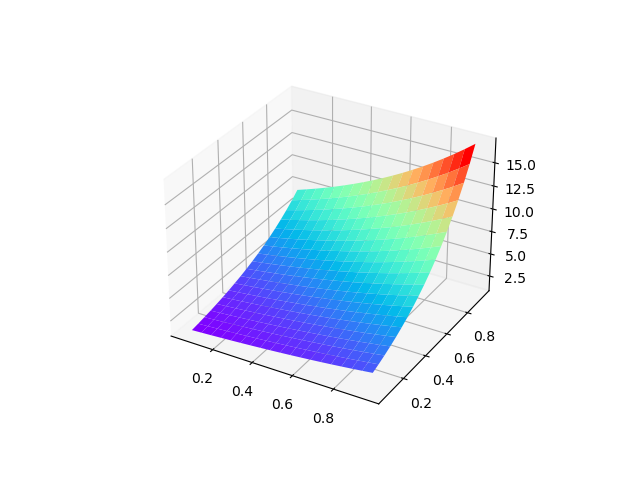
\includegraphics[width=0.7\textwidth]{result.png} %插入图片,[]中设置图片大小,{}中是图片文件名
    \caption{$h=0.05$结果图} %最终文档中希望显示的图片标题
    \label{Fig.main2} %用于文内引用的标签
\end{figure}
当取不同$h$,得到的误差如下表所示:

\begin{longtable}{ccc}
    \caption{不同$h$的误差表}\\\hline
    $h$ &  
    \multicolumn{1}{c}{误差}} \\\hline
    \endfirsthead
    \caption[]{不同$h$的误差表(续表)}\\
    \multicolumn{2}{r}{\footnotesize 接上页}\\\hline
    $h$ &  \multicolumn{1}{c}{误差}\\
    \hline\endhead
    \hline\multicolumn{2}{r}{\footnotesize 接下页}\\
    \endfoot\hline\hline\endlastfoot
    $\frac{1}{10}$ & 0.005519939625335368 \\
    $\frac{1}{20}$ & 0.0013997692884775148 \\
    $\frac{1}{40}$ & 0.0003511099859592193\\
    $\frac{1}{80}$ & 8.787626974093854e-05 \\
\end{longtable}

\end{document}